\begin{frame}
\frametitle{General Structure}
\begin{center}
	sim2d.cu

	\vspace{5mm}
	integrator.h
	
	integrator.cu
	\vspace{5mm}
	
	gl\_helper.cu
	
	gl\_helper.h
\end{center}
\end{frame}

\begin{frame}[fragile]
\frametitle{sim2d.cu}
Set: number of block, number of threads, other parameters.
\vspace{10mm}
\begin{lstlisting}
void readTiff(char *filename, float **raster, unsigned *w, 
		unsigned *h, float scale)
void step()

glutMainLoop()
\end{lstlisting}
\end{frame}

\begin{frame}[fragile]
\frametitle{integrator.cu}
\begin{lstlisting}
__global__ 
void stepSimulation2D(float *T, float *K, float *dT, 
			unsigned n_loop, uchar4 *tex, 
			char copy_tex)
__device__ 
void loadSharedMemory2D(const UsefulConstants consts, 
			float *T)
__device__ 
void integrate2D(const UsefulConstants consts, float *T, 
			float *K, float *dT)
\end{lstlisting}
\end{frame}

\begin{frame}[fragile]
\frametitle{loadSharedMemory2D}
\begin{lstlisting}
for (i = 0; i < n_loop; ++i) {
	local_T[lid_1d + i] = T[gid_1d + i];
	//d_operation[gid_1d+i] = 255;
}
__syncthreads();
\end{lstlisting}
\end{frame}

\begin{frame}[fragile]
\frametitle{loadSharedMemory2D}
\begin{center}
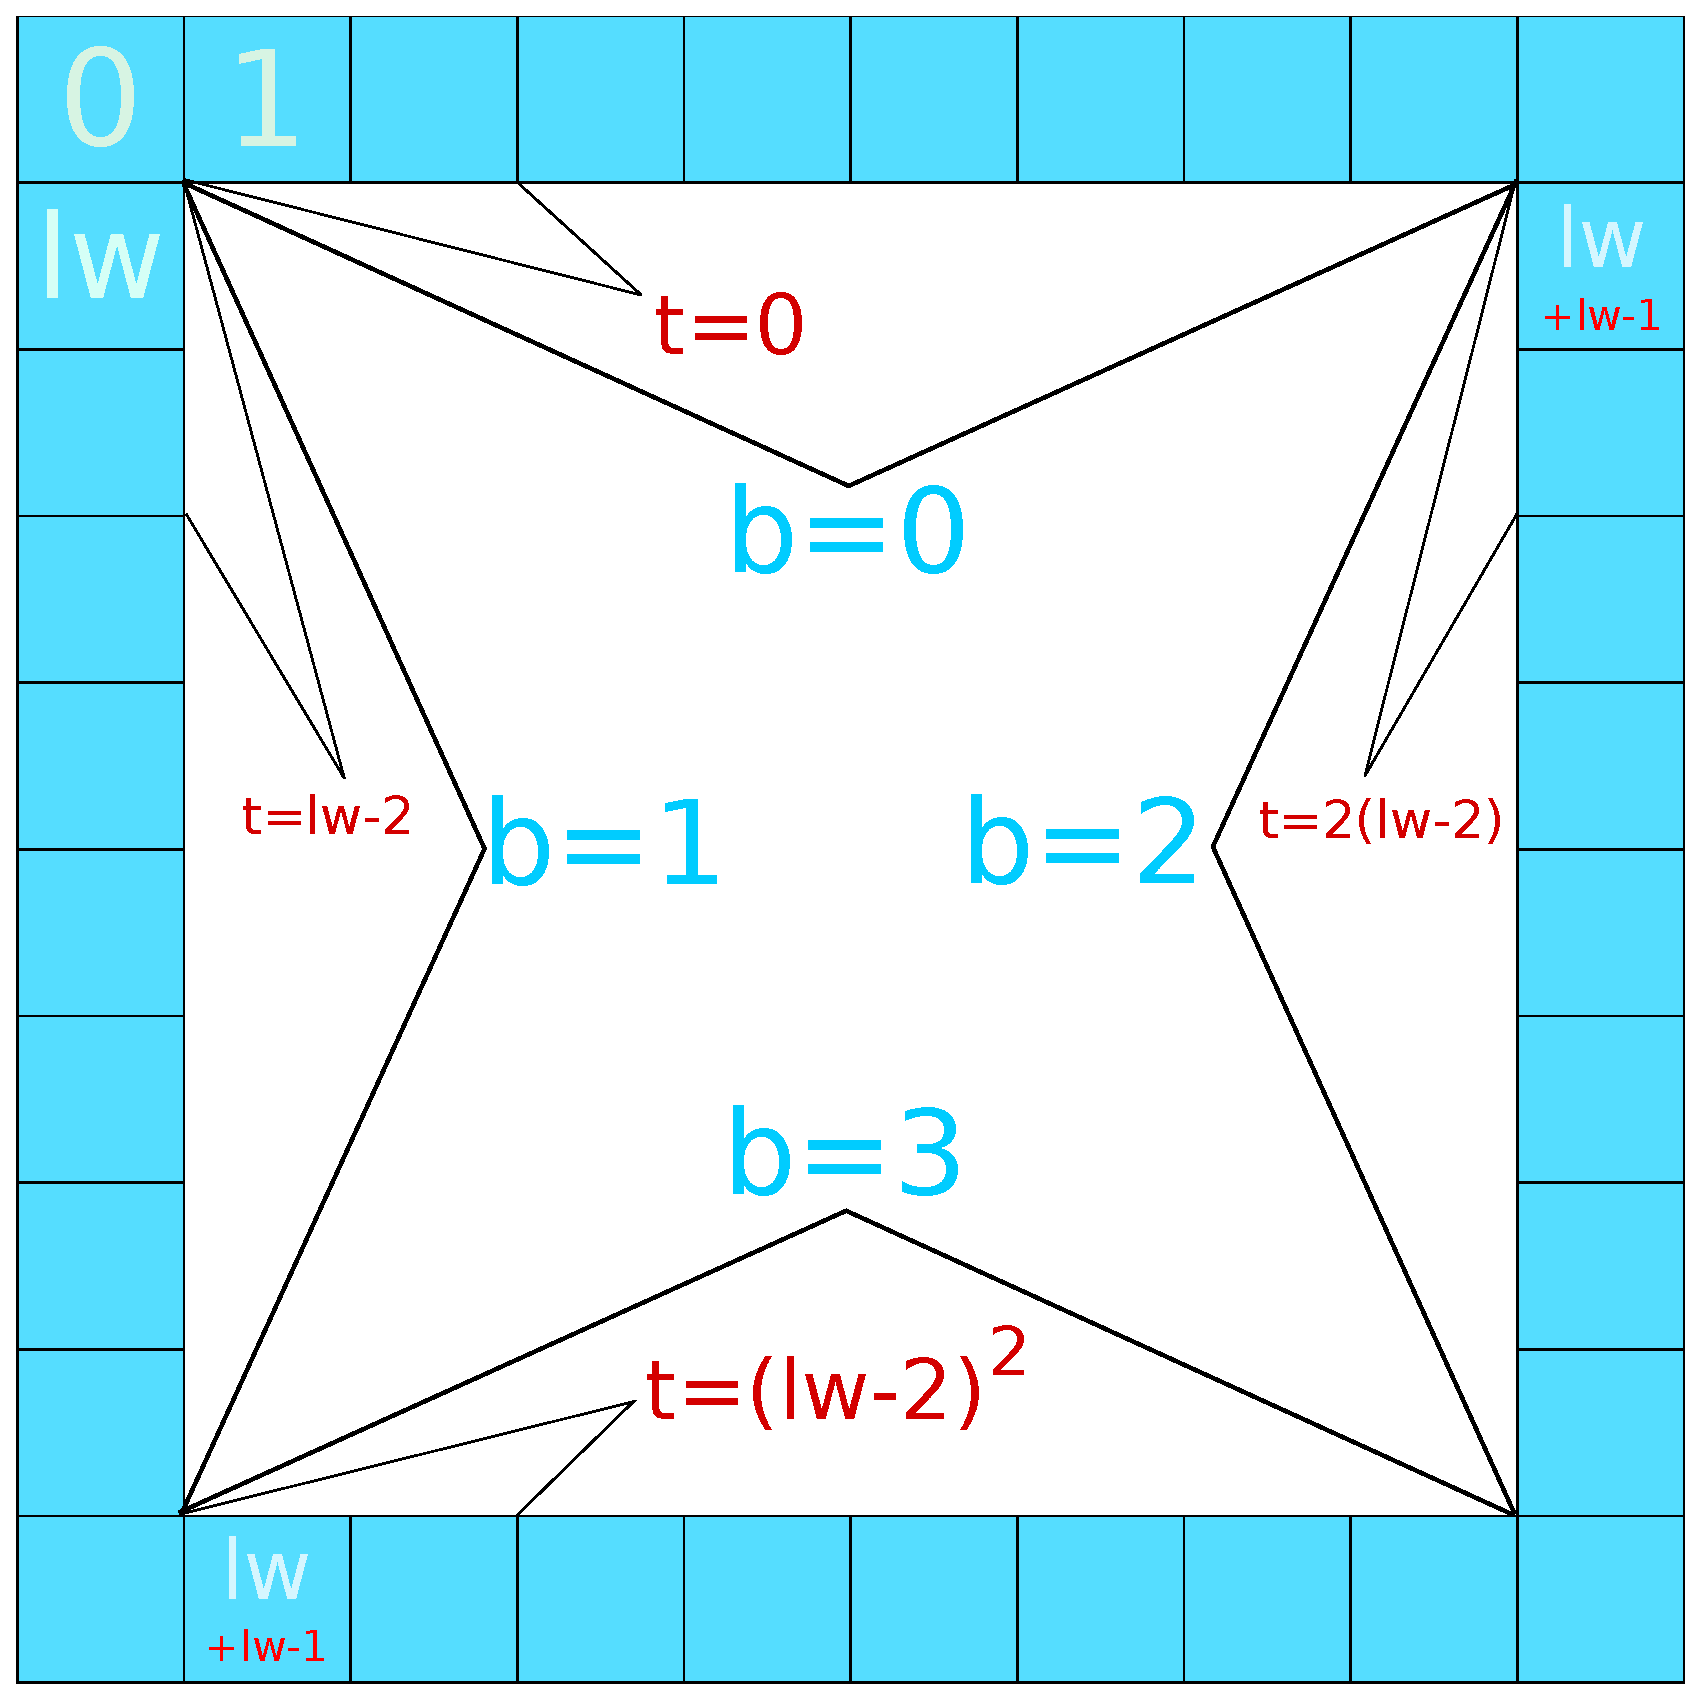
\includegraphics[scale=0.28]{images/borders.eps}
\end{center}
\end{frame}

\begin{frame}[fragile]
\frametitle{integrate2D}
\begin{lstlisting}
for (i = 0; i < consts.n_loop; ++i) {
	T[gid_1d+i] += K[gid_1d_nb+i] *
		(local_T[lid_1d+1+i] + local_T[lid_1d-1+i] 
		+ local_T[lid_1d+lw+i] + local_T[lid_1d-lw+i] 
		- 4*local_T[lid_1d+i])
		
		+ dT[gid_1d_nb+i];
}
\end{lstlisting}
\end{frame}


% Memory
\begin{frame}
\frametitle{Shared Memory}
\framesubtitle{Random errors}
\begin{center}

\includegraphics[scale=0.4]{../check/borders_1c_01.png}
\end{center}
\end{frame}


\begin{frame}
\frametitle{Shared Memory}
\framesubtitle{Synchronized threads}
\begin{center}

\includegraphics[scale=0.4]{../check/borders_sync.png}
\end{center}
\end{frame}